% =====================================================================
%  PÁGINA DO REGISTRO DE SOFTWARE (INPI)
%  --------------------------------------------------------------------
%  Inclui o certificado oficial de registro do programa de computador
%  emitido pelo INPI (Processo nº BR512026003786-7), que representa a
%  versão inicial do software Argus Cyclist. A evolução da versão
%  registrada para a versão apresentada neste trabalho é detalhada no
%  Capítulo~\ref{cap:registro-evolucao}.
%  =====================================================================

\thispagestyle{empty}

\noindent
\begin{minipage}{\textwidth}
  \begin{center}
    \textbf{\large REGISTRO DE SOFTWARE --- INPI}
    \vspace{0.8cm}
  \end{center}

  O software \argus{} foi registrado junto ao Instituto Nacional da
  Propriedade Industrial (INPI) sob o Processo nº
  \textbf{BR512026003786-7}, sendo o registro expedido em 02/06/2026. O
  registro foi realizado com base na \textbf{versão inicial} do sistema,
  desenvolvida na etapa inicial do projeto. O presente trabalho apresenta a
  \textbf{evolução} do \argus{} desde essa versão registrada até a versão
  atual, documentando aprimoramentos, novas funcionalidades e a
  consolidação da arquitetura do sistema.
\end{minipage}

\vspace{0.6cm}

\centerline{%
  \fbox{%
    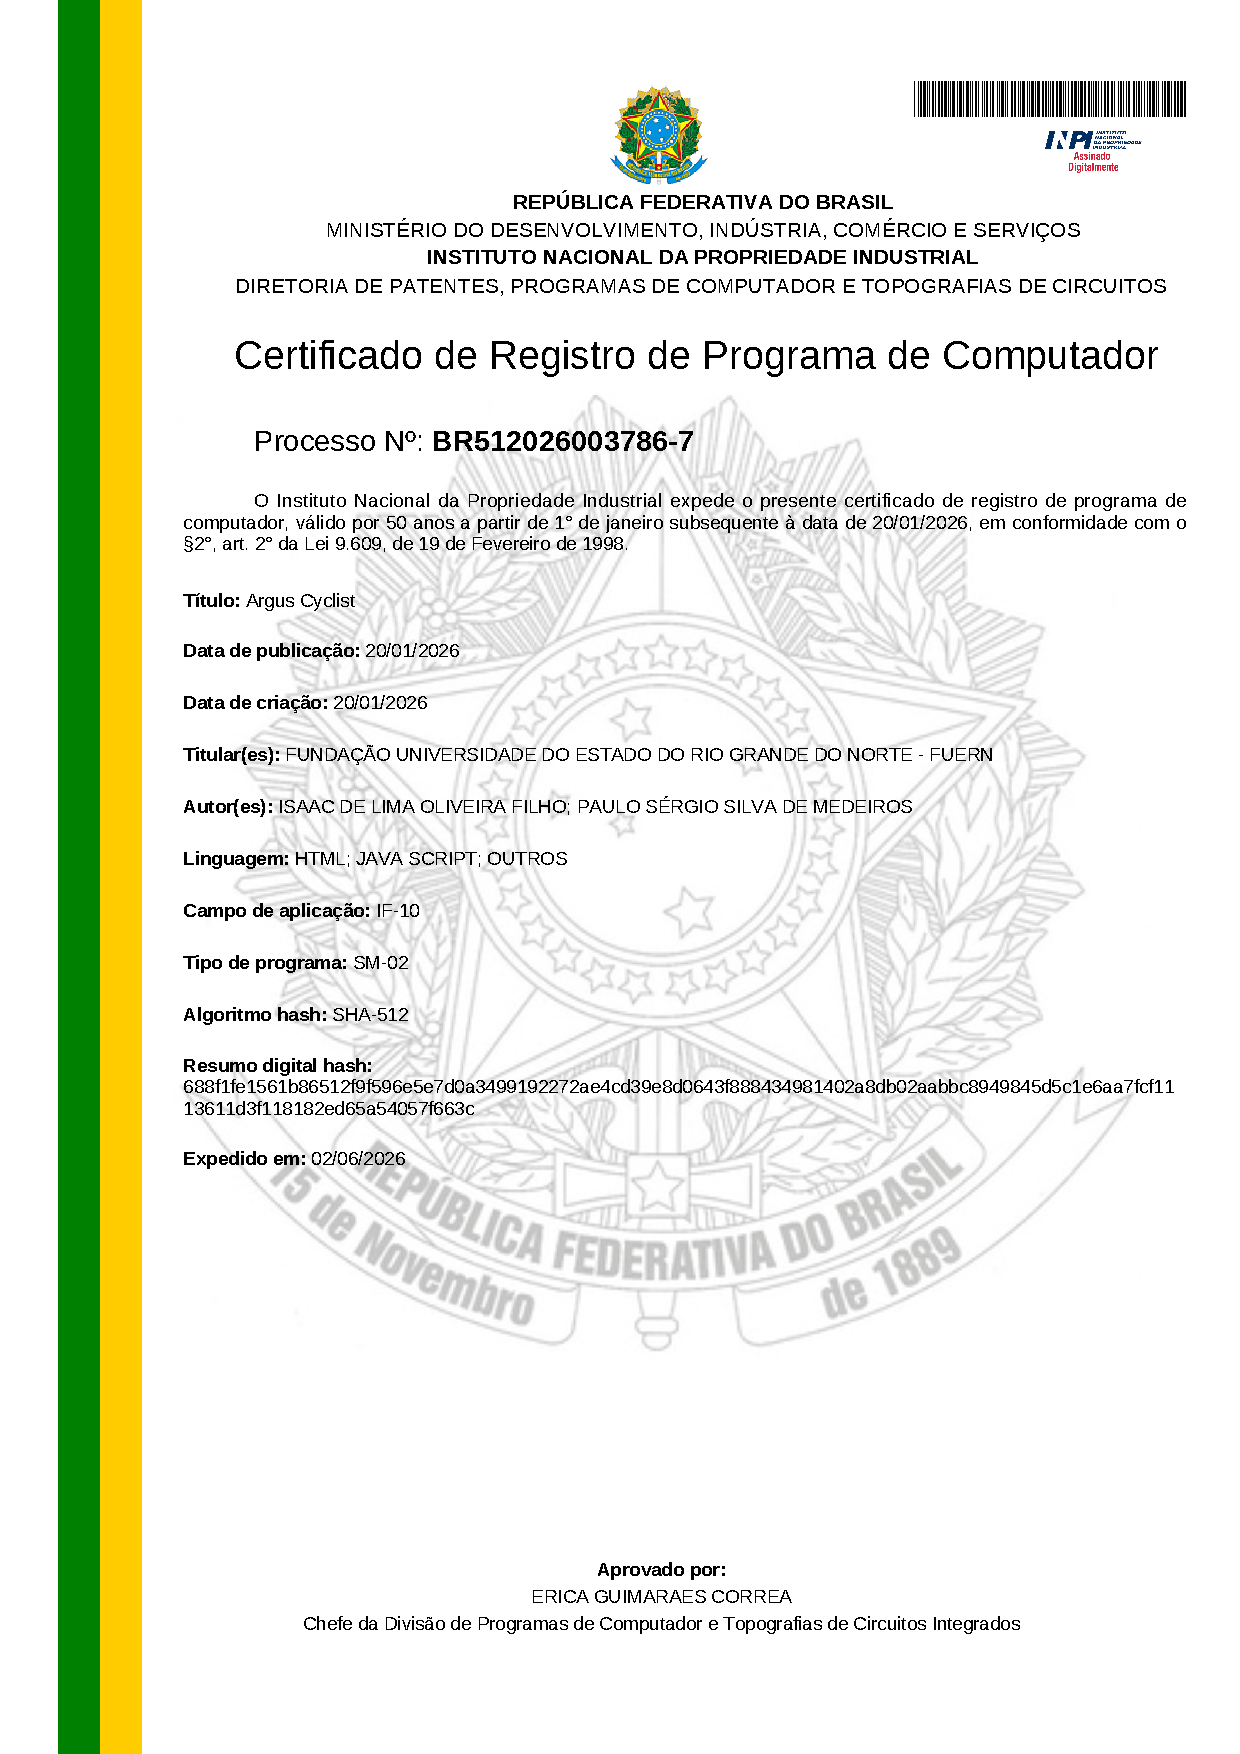
\includegraphics[width=0.75\textwidth,height=0.62\textheight,keepaspectratio]{certificado/certificado-registro-inpi.pdf}%
  }%
}

\vspace{0.6cm}

\begin{center}
  \small
  Certificado de Registro de Programa de Computador --- INPI
  \par
  Fonte: INPI (2026).
\end{center}

\newpage
